% Chapter Template

\chapter{Efficacy Transition Pathways} % Main chapter title

\label{etp} % For referencing this chapter elsewhere, use \ref{etp}

%----------------------------------------------------------------------------------------
%	SECTION 1
%----------------------------------------------------------------------------------------

\section{Introduction}
\label{etp:Introduction}

Phase \RN{2} trials build upon the work of early Phase \RN{1} trials where preliminary information is obtained regarding the safety profile and dose schedule of a treatment. The key output from a Phase \RN{1} trial is the MTD (Maximum Tolerated Dose), TD\%\% (target dose at some pre-specified level), RP2D (Recommended Phase \RN{2} Dose) or OBD (optimal biological dose) i.e. some dose-level that can be taken forward for future testing. In Phase \RN{2} trials the focus shifts away from toxicity and looks more towards efficacy of these new treatments at the dose-levels previously defined \cite{berryBayesianAdaptiveMethods2010}. The purpose of phase \RN{2} trials is to usually see if a new treatment or intervention works and establish if there is a efficacy signal. More specifically they aim to determine if there is a sufficient level of efficacy to warrant further research in for example a Phase \RN{3} setting \cite{juliousIntroductionStatisticsEarly2010}. In addition to assessing efficacy there is also opportunity to further explore the toxicity profile of the treatment as in comparison to Phase \RN{1} trials Phase \RN{2} trials are typically conducted using a larger sample size.  

Phase \RN{2} trials can be categorised further, dependent on the primary aims of the trial. Single-arm trials can be classified as Phase \RN{2} A trials, here a sample of patients would be given the experimental treatment and efficacy would be assessed. There are also multi-arm trials which may randomise patients to multiple experimental treatments or between an experimental treatment and standard of care. Efficacy would then be compared across the different arms. These types of trials are commonly referred to as Phase \RN{2} B trials. 

Generally speaking Phase \RN{2} trials should be efficient and quick such that we can progress to Phase \RN{3} as quickly as possible or drop any ineffective treatments. The output from a Phase \RN{2} trial should be either a 'GO' or 'No GO' decision i.e should we or should we not proceed to later phase testing based on the data observed in this trial. One of the more important aspects of these trials is that we don't want to make any incorrect decisions and if there is an effective treatment that is being investigated we want to make sure that it is taken forward into Phase \RN{3}.

An example of a Phase II single arm trial design is depicted in Figure \ref{fig_etp:phase2_singlearm_example}. For single-arm Phase \RN{2} trials eligible patients come into the trial and all of them will be allocated to the new treatment. Once they have completed their treatment period we would then assess the effectiveness of that treatment using some measure of success. Looking at the outcome of success in each patient the success rate or proportion of success can then be determined. In the single arm setting, this success rate is then compared to some sort of benchmark, which is determined from either historical data or clinical input.


\begin{figure}[h!]
	\centering
	\caption{Example of a Phase 2 single arm trial design.}
	\label{fig_etp:phase2_singlearm_example}
	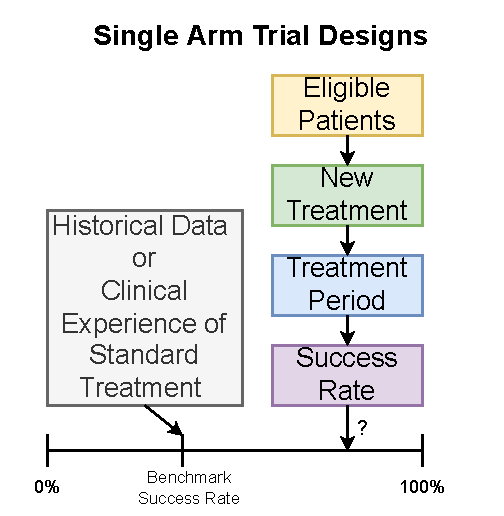
\includegraphics[width=0.75\textwidth]{ETP-Phase2SingleArmExample}
\end{figure}

The primary outcome measure for a trial like this should be some short-term binary outcome either success or failure. The outcome measure selected should be chosen such that you expect the treatment to have an effect on that. Typically these are surrogates for longer-term efficacy measures. So, if we see a success in the Phase II trial we would hope there would also be some long-term benefits for patients as well. In the oncology setting Phase III trials typically will look at outcomes such as survival times but in the previous Phase II trials response or change in tumour size may have been used as outcomes.

There are many classical frequentist approaches which can be applied to Phase \RN{2} trials such as the Flemming A'Hern, Simons two-stage or Bryant and Day designs. However, there exist complex and innovative designs that are adaptive in nature and allow for more frequent interim analyses so decisions can be made faster. 

One approach is Bayesian and utilises a Beta-Binomial conjugate analysis to estimate a  response rate for a binary outcome. Posterior probabilities can be used to inform decision making and predictive probabilities can be used during interim analyses in a similar manner. This is typically done using pre-specified decision rules.

Whilst mathematically simple to implement a design such as this has similar drawbacks to dose-finding methodologies that have been previously discussed. Due to its flexibility there may be some issues with parametrising the design, in this case would mean selecting the correct decision rules. A Bayesian approach may be less familiar than traditional frequentist approaches that are more commonly used. It may also be hard to understand why certain decisions are being made during interim and final analyses.  

One potential solution to these problems was devised by Lucinda Billingham who developed Efficacy Transition Pathways (ETPs) a novel visualisation tool to aid the design and interpretation of these types of trial designs. ETPs extend on the idea of dose transition pathways, which solves for many of the same issues in dose-finding trials. 

In this chapter we will explore the components that go into constructing an ETP for a Beta-Binomial conjugate analysis. We will detail how ETPs can be used in a trial setting with an illustrative example. Finally, we also provide details on a web application that can be used to produce ETPs and acts as an educational tool to explain what they are. 

%----------------------------------------------------------------------------------------
%	SECTION 2
%----------------------------------------------------------------------------------------

\section{Beta-Binomial Conjugate Analyses}

Bayesian methods are an alternative way of thinking about evidence, data and statistics compared to the traditional frequentist approach. The Bayesian approach could be considered more intuitive and has some advantages that make it useful for analysing clinical trials. 

The fundamentals of Bayesian statistics are well defined in the literature as well as its application to clinical trials and health research. Bland and Altman \cite{blandBayesiansFrequentists1998} discuss the differences between a Bayesian or a frequentist approach. Spiegelhalter et al. \cite{spiegelhalterIntroductionBayesianMethods1999} detail the underlying philosophy behind Bayesian methods along with its application in health technology assessment. General Bayesian methods are described in more detail in books by Lee \cite{leeBayesianStatisticsIntroduction2012} and Bernado and Smith \cite{bernardoBayesianTheory2009}. It should be noted, these are just a few examples from the literature.    

The Bayesian paradigm doesn’t regard parameters, things we don’t know like a treatment effect ($\theta$), as fixed. These are instead thought of to be uncertain. Bayesian statistics uses probability to express this uncertainty. Since $\theta$ is unknown, it has a probability distribution. 

Bayesian analysis takes into account prior information on $\theta$ which also has the form of a probability distribution. This is combined with the likelihood of the data, Y given $\theta$, to produce a posterior probability distribution of $\theta$ given Y. So, data is collected to find out about the parameter. This data can be regarded as known and fixed and is used to estimate the unknown parameter. In Bayesian statistics, we estimate the probability of the parameter given the data.

Once a posterior distribution is established inferences can then be made about $\theta$. However, this may require numerical integration of the posterior distribution which may be difficult or impossible to evaluate analytically. An option around this is to use conjugate priors. If the posterior distribution and the prior distribution are from the same probability distribution family these can be referred to as conjugate distributions and the prior as a conjugate prior. Conjugate priors are algebraically easier to deal with and allow for easier interpretation of the posterior distribution. 

One example of this is what is commonly referred to as the Beta-Binomial conjugate. This is where the prior and posterior distributions take the form of a Beta distribution and the likelihood or data is Binomial. 

Binomial data has two possible outcomes. For example, a coin toss has two outcomes either its head or its tails. In the context of a Phase II single arm trial, this could be either a success/failure to some new treatment or response/no response. When this is combined with a Beta prior distribution we get a posterior Beta distribution. From this, we can then make probability statements about the treatment effect.

Following the explanation by Lee \cite{leeBayesianStatisticsIntroduction2012} of a Beta conjugate prior for a binomial distribution. Consider a parameter of interest $\theta$ that represents some treatment effect. More specifically, for binomial data in a single arm Phase \RN{2} clinical trial, lets say the parameter $\theta$ is the probability of response in a number of patients following a some new treatment. Each patient can experience either a response or no response, with the same probability of response and each patient being independent from each other. For a fixed sample size with $n$ patients and number of responses ($y$) we have: 

\begin{equation}
	y \sim \text{Binomial}(n, \theta)
\end{equation}

So, $y$ is from a binomial distribution which produces the following likelihood: 

\begin{equation}
	L(\theta) = P(y|\theta) = {n \choose y}\theta^y (1-\theta)^{n-y} \; \; \; \; (y = 0,1,\ldots,n)
\end{equation}

If the prior for $\theta$ is from a Beta distribution such that 

\begin{equation}
	P(\theta) = \text{Beta}(a,b)
\end{equation}

then the posterior distribution is also from a Beta distribution and can be expressed as 

\begin{equation}
\label{eq_etp:betaposterior}
	P(\theta|y) = \text{Beta}(a+y,b+n-y)
\end{equation}

To avoid confusion with the prior we will let $\alpha = a+y$ and $\beta = b+n-y$ which gives

\begin{equation}
	\label{eq_etp:betaposterior2}
	P(\theta|y) = \text{Beta}(\alpha,\beta)
\end{equation}

Bayesian inference can then be used for estimation and decision making. Features such as the mean and  variance of the treatment effect $\theta$ can be  estimated from the posterior distribution given in equation \ref{eq_etp:betaposterior2}. For the posterior distribution of $\theta \sim Beta(\alpha,\beta)$ the mean, variance and mode are.

\begin{equation}
\label{eq_etp:betamean}
	E[\theta] = \frac{\alpha}{\alpha + \beta} 
\end{equation}

\begin{equation}
\label{eq_etp:betavar}
	Var[\theta] = \frac{\alpha\beta}{(\alpha+\beta)^2 (\alpha+\beta+1)}
\end{equation}

\begin{equation}
	\label{eq_etp:betamode}
	mode[\theta] = \frac{\alpha - 1 }{\alpha + \beta - 2} 
\end{equation}
 
The proofs for these formula are relatively simple and can be found in \cite{sochBookStatisticalProofs2020}. There exists no closed formula for the median however this can still be calculated using the density function of a Beta distribution. If we take $\theta^m$ to be the median then, the median is the value that solves 

\begin{equation}
	P(\theta < Median) = 0.5 = \int_{0}^{\theta^m} \theta^{\alpha-1}(1-\theta)^{\beta-1}d\theta
\end{equation}

Alternatively, there is a closed form approximation to the median presented by Kerman \cite{kermanClosedformApproximationMedian2011} which is as follows 

\begin{equation}
	median[\theta] \approx \frac{\alpha - \frac{1}{3}}{\alpha + \beta - \frac{2}{3}}
\end{equation}

We can also establish credible intervals or make other probability statements in a similar manner. 
Then pre-specified rules based on these direct probabilities from the posterior can be used for decision making purposes. For example, if 

\begin{equation}
	P(\theta > c |y) \geq q  \; \; \; \; \text{then GO else No GO}
\end{equation}


where $c$ is some target level of treatment effect and $q$ is some threshold of sufficient evidence. This probability can be calculated from the density function of the Beta distribution from $c$ to $\infty$. 

\begin{equation}
	P(\theta > c | y) = \int_{c}^{\infty}\theta^{\alpha-1}(1-\theta)^{\beta-1}d\theta
\end{equation}

It should be noted that $\int_{0}^{1}\theta^{\alpha-1}(1-\theta)^{\beta-1}d\theta = 1$, so $\theta$ has an upper bound of 1. Appropriate decision criteria, i.e. values for $c$ and $q$, can be determined and evaluated via simulations.

%-----------------------------------
%	SUBSECTION 1
%-----------------------------------

\subsection{Illustrative example to showcase a Beta-Binomial design} 
In this section we will detail an example to show how a Beta-Binomial conjugate analysis would work in practice and how its used to make decisions. 

Consider a trial in which we are trying to evaluate the efficacy of some new treatment. This will be done using an outcome measure of response. Patients can either be considered a responder or a non-responder. The treatment effect will be the response rate and will be analysed using a Beta-Binomial conjugate model. 

To conduct the analysis and make a GO or No GO decision a prior and decision criteria needs to be specified. For simplicity a minimally informative $Beta(1,1)$ prior will be used. This represents a 50\% response rate from a group of two patients. The following decision rule will also be used $P(\theta  \geq 30\%) \geq 0.9$, where $\theta$ is the treatment effect (response rate). So, if there is a greater than  90\% chance that the true response rate is at least 30\% this will be considered sufficient evidence to warrant a GO decision. 

Now assume that 30 patients were recruited 16 of which had a response. Using equation \ref{eq_etp:betaposterior} we can establish that the posterior distribution for the treatment effect is $P(\theta) = Beta(17, 15)$. From this we can then calculate summary estimates, which are presented in Table \ref{tab_etp:bb_sum_est}.

\begin{table}[H]
	\centering
	\caption{Summary estimates of response rate with 30 patients and 16 responses. }
	\label{tab_etp:bb_sum_est}
	\begin{tabular}{cc}
		\hline
		\textbf{Summary Estimate}                   &              \\ \hline
		\multicolumn{1}{c|}{Mean}                   & 0.531        \\
		\multicolumn{1}{c|}{Median}                 & 0.532       \\
		\multicolumn{1}{c|}{Mode}                   & 0.533          \\
		\multicolumn{1}{c|}{Variance}               & 0.008        \\
		\multicolumn{1}{c|}{95\% Credible Interval} & 0.360, 0.698 \\ \hline
	\end{tabular}
\end{table}

From these estimates we can say, based on the data that is observed (16 responses in 30 patients), the response rate is 53\% with a 95\% credible interval (36\%, 70\%). The probability of the response rate being at least 40\% can also be calculated. In this example it is 99.7\%. As this value is greater than the threshold of 90\%  we can say there is sufficient evidence to warrant a GO decision.

This can also be illustrated as shown in Figure \ref{fig_etp:bb_dec_rule1}. The blue shaded region highlights the upper 90\% of the distribution. In this scenario with this decision criteria, as the entire region does not cross the target response rate of 30\% we have a GO decision. We can see that there is a greater than 90\% chance that the response rate is greater than 30\%. 

 \begin{figure}[h!]
 	\centering
 	\caption{Posterior distribution of response rate with decision criteria.}
 	\label{fig_etp:bb_dec_rule1}
 	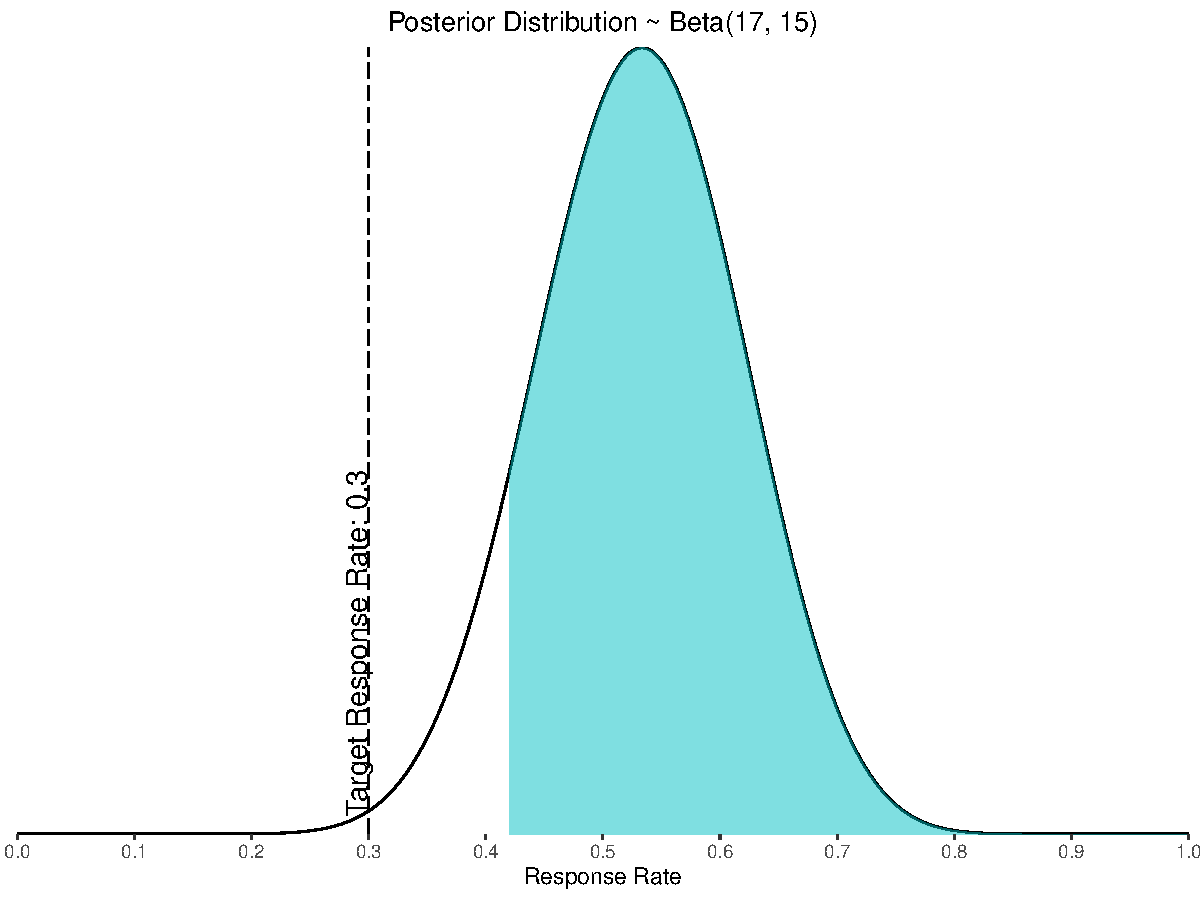
\includegraphics[width=\textwidth]{ETP-BetaBinomialDecRule1}
 \end{figure}

In practice decision rules should be decided before the trial starts. This is typically done via the evaluation of simulations. Multiple scenarios corresponding to different true response rates can be investigated. The probability of making a correct decision can then be calculated. This represents the power of our design. For scenarios with low true response rates (relative to the target response rate) we want the probability of making a No GO decision to be high. Similarly, for scenarios with high true response rates we want the probability of making a GO decision to be high. The decision rule parameters, the target response rate and probability threshold can then be adjusted to ensure the design is making appropriate decisions in these scenarios. 

Simulations can also be used to evaluate the choice of prior as well. A variety of different priors can be used dependent on the trial. A prior like the Beta(1,1) is typically described as minimally informative. This means that if the data observed is reasonably large the likelihood will dominate and have more influence on the posterior. So, if we observe a really strong treatment effect this will be reflected in the posterior. 

A sceptical prior can be used when we are sceptical about the treatment producing large treatment effects. These are typically centred around a low treatment effect whilst still leaving some scope for their to be plausible positive treatment effect. The opposite of this would be a enthusiastic prior. Here the prior would be centered around a high treatment effect whilst allowing some possibility for a negative treatment effect.

Priors can also be evidence based or elicited. Evidence based priors will use results or data from previous trials to inform the choice of prior. These can then be adjusted to account for any potential biases. Elicited priors are decided based on discussions with a group of experts. 

Figure \ref{fig_etp:bb_example_priors} shows the effect that different priors can have on the estimation of the treatment effect. Our example with 16 responses and a minimally informative prior is shown in the first plot. Here we can see the median response rate is 53.2\% and the probability of the response rate being greater than 30\% is greater than 90\% meaning we have a go decision. The minimally informative prior is indicated by the red line and is essentially a uniform distribution. Assuming we still have 16 responses, we can see that when a sceptical $Beta(2,8)$ prior is implemented the posterior distribution changes from $Beta(17,15)$ to $Beta(18,22)$. This shifts the posterior such that the new estimated median response rate is 44.9\%. However even with a sceptical prior we can still see we meet the criteria for a GO decision with a probability of 0.976 that the response rate is greater than 30\%. Then with an enthusiastic prior the posterior shifts in the other direction. So, with the same 16 responses but an enthusiastic prior the estimate of the response rate is 57.6\%. Again, the decision criteria is also met in this instance as well.    

 \begin{figure}[h!]
	\centering
	\caption{Posterior distribution of example under different priors.}
	\label{fig_etp:bb_example_priors}
	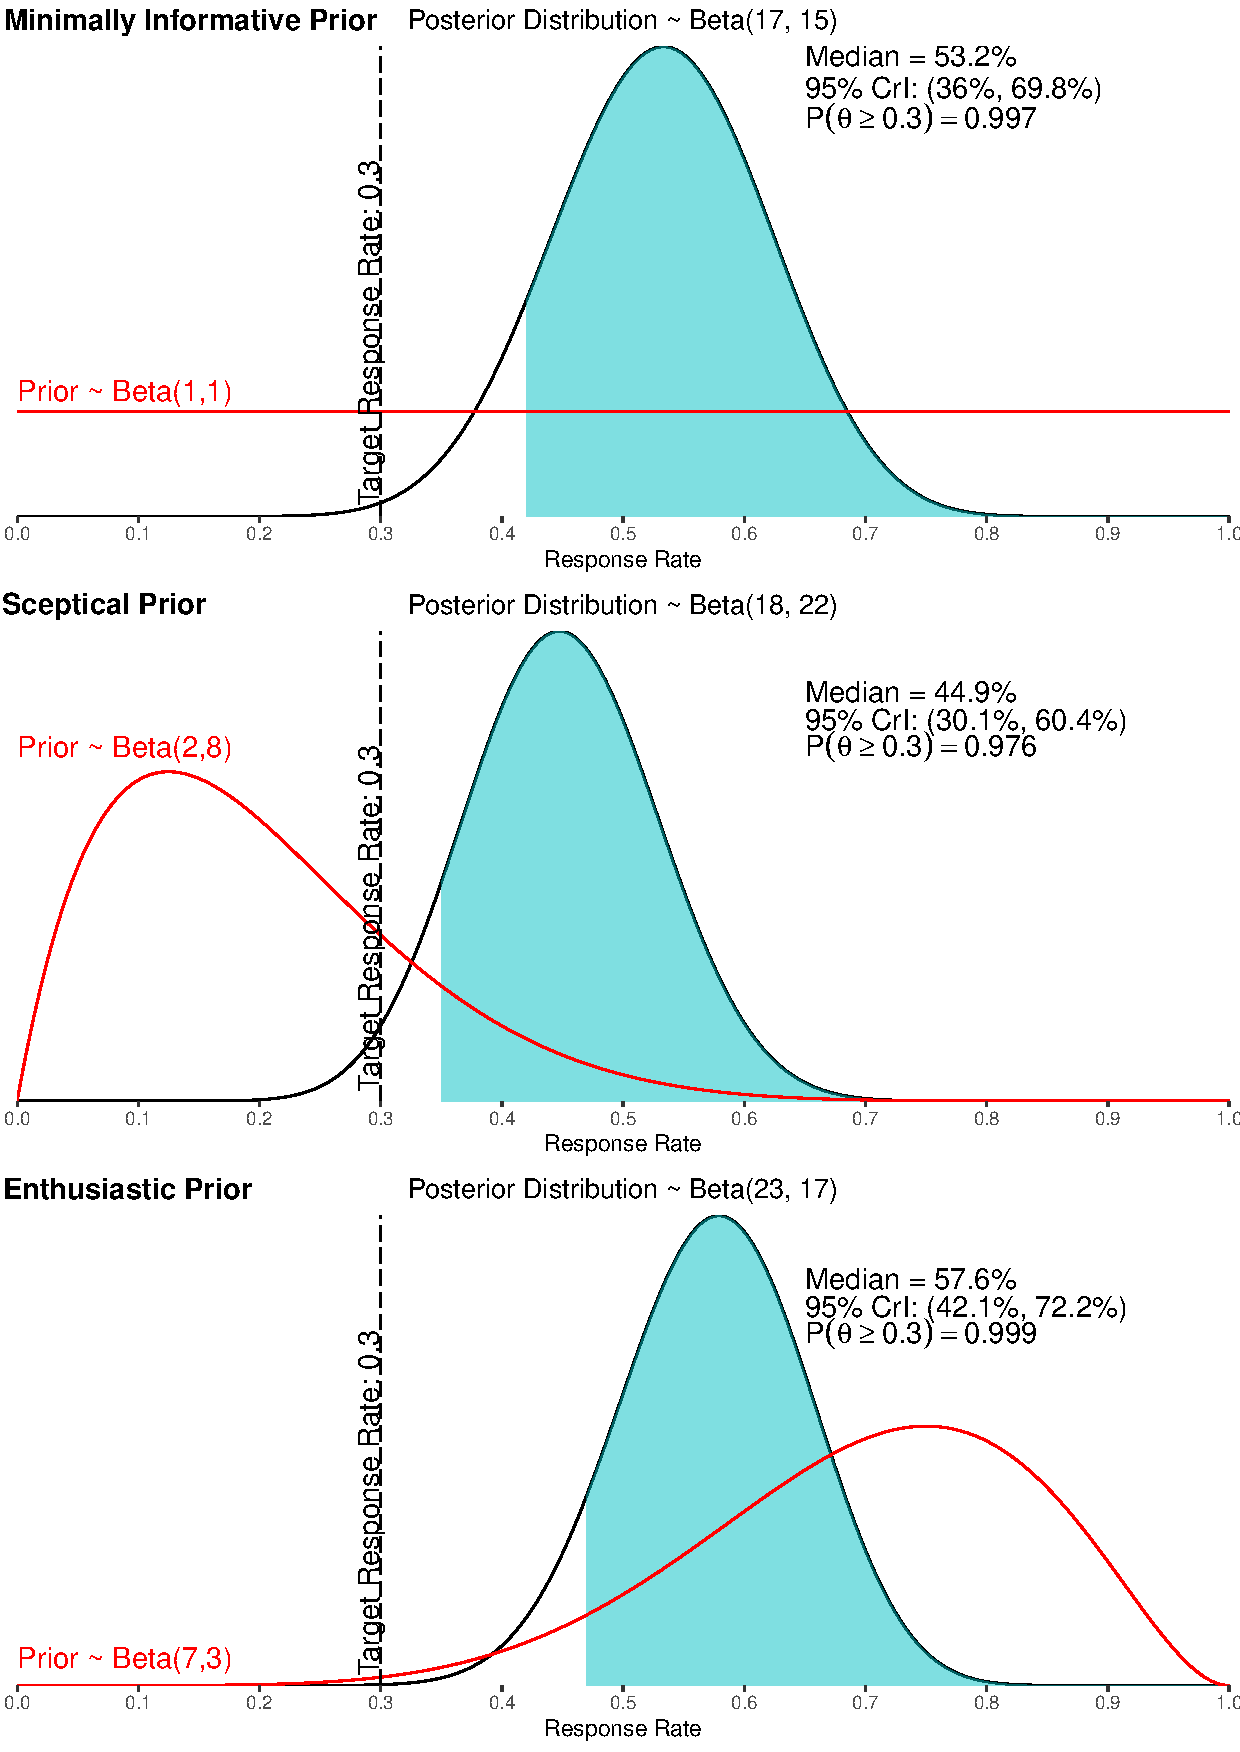
\includegraphics[width=\textwidth]{ETP-BetaBinomialPriors}
\end{figure}

In this example the choice of prior did not impact the decision that would be made. However, if the decision rule was different or the number of responses seen was less this could change. As part of some trials a sensitivity may be conducted to check the results and decisions of a trial with a different prior. As stated before simulation work is used to establish the most appropriate decision criteria and priors can be sourced from available evidence or elicited. The simulations should be conducted with the priors in mind as well as any sensitivity analyses that may be planned.   

Once the decision rule and prior have been specified the minimum number of responses required to make a GO decision could also be calculated. In our example here this number is 12. So, we would need to observe a minimum of 12 responses to make a GO decision out of 30 patients. As the Beta-Binomial conjugate analysis is Bayesian in nature we can make use of this information and incorporate interim analyses into the trial. This would work by evaluating the data at pre-specified time points or after a certain amount of patients have been recruited. At these time points we can determine whether or not we have observed enough responses to warrant continuing with the trial based on the overall minimum responses we would need for a final GO decision. This is typically referred to as the predictive probability of success (PPOS). In the next section we look at how the PPoS is used to make decisions at interim analyses. 

%-----------------------------------
%	SUBSECTION 3
%-----------------------------------

\subsection{Interim analyses and Predictive Probability of Success}

%----------------------------------------------------------------------------------------
%	SECTION 3
%----------------------------------------------------------------------------------------

\section{Constructing Efficacy Transition Pathways}

%-----------------------------------
%	SUBSECTION 1
%-----------------------------------

\subsection{Application the DETERMINE trial}

%----------------------------------------------------------------------------------------
%	SECTION 4
%----------------------------------------------------------------------------------------

\section{Development of a Web Application for ETPs}